% 原书 p.244–p.246（PDF p.252–p.254）
% 第 9 章 9.3 节：拉格朗日子流形之间的距离（小尺度）

% >>> p252
\section{拉格朗日子流形之间的距离（小尺度）
（Distance Between Lagrangians (Small Scale)）}

\begin{keytakeaways}
\begin{itemize}
  \item 几何图像：辛同胚群 $\Ham(M,\omega)$ 作用在给定子流形 $L$ 的轨道空间
        $\mathcal O(L)$ 上；$\Ham$ 上的共轭不变范数（如 Hofer 范数）在轨道空间上
        诱导伪度量 $\delta_{\|\cdot\|}$，它度量「把 $L_1$ 搬到 $L_2$ 需要多大的
        哈密顿能量」。
  \item 数学工具：共轭不变范数、稳定化子 $\operatorname{Stab}(L)$、刚性轨迹
        $R_L$（定义 9.3.1）、Banyaga 碎片化引理（引理 9.3.2）。
  \item 本节结论：二歧性定理 9.3.1——对 Hofer 范数，$\delta_{\|\cdot\|}$ 要么非退化，
        要么恒为零；且 $\delta_{\|\cdot\|}$ 非退化当且仅当 $R_L=L$（观察 (iii)）。
\end{itemize}
\end{keytakeaways}

给定闭连通子流形 $L^n\subset(M^{2n},\omega)$，经由 $\Ham(M,\omega)$ 的作用，我们得到
轨道空间
\begin{equation*}
  \mathcal O(L):=\bigl\{\varphi(L)\subset M\mid\varphi\in\Ham(M,\omega)\bigr\},
\end{equation*}
其中按定义 $\Ham(M,\omega)$ 在 $\mathcal O(L)$ 上传递地作用。这里有一个基本观察：
$\Ham(M,\omega)$ 上任何共轭不变范数 $\|\cdot\|$（例如 6.1 节定义的 Hofer 范数
$\|\cdot\|_{\mathrm{Hofer}}$）在 $\mathcal O(L)$ 上诱导一个伪度量
\begin{equation}\tag{9.20}
  \delta_{\|\cdot\|}(L_1,L_2)
  :=\inf\bigl\{\|\varphi\|\mid\varphi\in\Ham(M,\omega),\ \varphi(L_1)=L_2\bigr\}.
\end{equation}
对任意 $L_1,L_2\in\mathcal O(L)$。由于 $\Ham(M,\omega)$ 在 $\mathcal O(L)$ 上的作用
是传递的，总可以假设 $L_1$ 或 $L_2$ 为「基点」$L$。
% [Tutor Note: 易错预警——$\delta_{\|\cdot\|}$ 一般只是\emph{伪}度量：非退化性
% （即 $L_1\neq L_2$ 蕴含 $\delta(L_1,L_2)>0$）并非自动成立，这正是练习 9.3.1 与
% 定理 9.3.1 讨论的核心。又「共轭不变」指 $\|\psi\varphi\psi^{-1}\|=\|\varphi\|$，
% 它保证 $\delta$ 在 $\Ham(M,\omega)$ 作用下不变，从而不依赖于基点 $L$ 的选取。]

下文将频繁出现的一个关键概念是 $\Ham(M,\omega)$ 在 $\mathcal O(L)$ 上作用的
\textbf{稳定化子}：
\begin{equation}\tag{9.21}
  \operatorname{Stab}_{\|\cdot\|}(L)
  :=\bigl\{\varphi\in\Ham(M,\omega)\mid\varphi(L)=L\bigr\}.
\end{equation}
下面的练习表明，$\mathcal O(L)$ 上的 $\delta_{\|\cdot\|}$ 与
$\operatorname{Stab}_{\|\cdot\|}(L)$ 密切相关。

% >>> p253
\begin{wexer}{9.3.1}
  证明：$\delta_{\|\cdot\|}$ 非退化，当且仅当由 (9.21) 定义的稳定化子
  $\operatorname{Stab}_{\|\cdot\|}(L)$ 是 $\Ham(M,\omega)$ 的真闭子集。这里非退化
  指对任意 $L_1\neq L_2\in\mathcal O(L)$ 都有 $\delta_{\|\cdot\|}(L_1,L_2)>0$；
  $\Ham(M,\omega)$ 上的拓扑由范数 $\|\cdot\|$ 诱导。
\end{wexer}
% [Tutor Note: 含糊点拨——练习 9.3.1 的两个方向分别对应「闭合性」与「非退化性」：
% 若 $\delta(L_1,L_2)=0$，可取 $\varphi_n$ 使 $\varphi_n(L_1)=L_2$ 且
% $\|\varphi_n\|\to0$，利用 $\Ham(M,\omega)$ 在该范数下的完备性得到把 $L_1$ 搬到
% $L_2$ 的极限元素，从而说明稳定化子不闭；反之，若稳定化子不闭，取
% $\varphi_n\in\operatorname{Stab}(L)$ 收敛到 $\varphi\notin
% \operatorname{Stab}(L)$，用共轭不变性 $\|\psi\varphi\psi^{-1}\|=\|\varphi\|$
% 可把相应的能量压到 $0$，得到 $\delta(L,\varphi(L))=0$。两步都用到范数的共轭
% 不变性与 $\Ham$ 的完备性，原文留给读者补全。]

当 (9.20) 中的共轭不变范数 $\|\cdot\|$ 取为 Hofer 范数
$\|\cdot\|_{\mathrm{Hofer}}$ 时，关于 $\delta_{\|\cdot\|}$ 有下面这个奇特的结果。
它是辛几何与切触几何中众多二歧性（dichotomy）型结果之一。

\begin{wthm}{9.3.1}（[47] 中的定理 2，[226] 中的推论 2.7）
  设 $(M,\omega)$ 是 $2n$ 维辛流形，$\|\cdot\|$ 是 $\Ham(M,\omega)$ 上的 Hofer
  范数。则对任意闭连通子流形 $L^n\subset M$，诱导的伪度量
  $\delta_{\|\cdot\|}$ 要么非退化，要么在 $\mathcal O(L)$ 上恒为零。
\end{wthm}

\begin{wrem}{9.3.1}
  事实上，由 [47] 中的定理 1，若 $L^n\subset M^{2n}$ 是拉格朗日子流形，则
  $\delta_{\|\cdot\|}$ 确实非退化。这基于对伪全纯曲线的一些分析（例如参见 [225]
  中的定理 4.9）。有趣的是，其逆命题也成立，且论证的技术性不高，因此我们把它留作
  下面的练习。
\end{wrem}

\begin{wexer}{9.3.2}
  设 $L^n\subset M^{2n}$ 是闭连通子流形。证明：若 $\delta_{\|\cdot\|}$ 在轨道空间
  $\mathcal O(L)$ 上非退化，则 $L$ 是拉格朗日子流形。
\end{wexer}

定理 9.3.1 有几个独立的证明。这里我们给出的论证依赖于 [225] 中引入的如下概念。

\begin{wdefn}{9.3.1}
  给定闭子流形 $L^n\subset(M^{2n},\omega)$，$L$ 的\textbf{刚性轨迹}
  （rigid locus）为
  \begin{equation}\tag{9.22}
    R_L:=\bigcap_{\varphi\in\overline{\operatorname{Stab}}_{\|\cdot\|}(L)}
    \varphi^{-1}(L),
  \end{equation}
  其中 $\overline{\operatorname{Stab}}_{\|\cdot\|}(L)$ 是 $L$ 的稳定化子在
  $\Ham(M,\omega)$ 中的闭包，所取的拓扑由范数 $\|\cdot\|$ 诱导。
  \hfill$\square$
\end{wdefn}
% [Tutor Note: 术语依据——rigid locus 译作「刚性轨迹」，与「刚性（rigidity）」的
% 用法一致；它一般不是流形（见注 9.3.4），只是闭子集，因此这里不用「子流形」。
% (9.22) 中的交取遍稳定化子\emph{闭包}中的元素，这一步是必要的：若只对
% $\operatorname{Stab}(L)$ 本身取交，所得集合总包含 $L$ 而无从探测非退化性。]

为简洁起见，一旦共轭不变范数 $\|\cdot\|$ 固定，我们就把
$\operatorname{Stab}_{\|\cdot\|}(L)$ 记作 $\operatorname{Stab}(L)$。由定义 9.3.1，
我们有如下观察。
\begin{enumerate}[label=(\roman*)]
  \item 集合 $R_L\subset M$ 是闭子集，因为 $L$ 是闭子流形。
  \item 此外 $R_L\subset L$，因为我们总可以在 $\operatorname{Stab}(L)$
    中取 $\varphi=\mathbf 1$。
  \item 我们有 $R_L=L$，当且仅当 $\delta_{\|\cdot\|}$ 非退化。
\end{enumerate}

% >>> p254
\begin{wproof}[观察 (iii) 的证明]
  若 $\delta_{\|\cdot\|}$ 非退化，则由练习 9.3.1，
  $\overline{\operatorname{Stab}(L)}=\operatorname{Stab}(L)$。由定义 9.3.1，
  $R_L=L$，因为此时任意 $\varphi\in\overline{\operatorname{Stab}(L)}$ 都满足
  $\varphi(L)=L$。
  另一方面，若 $\delta_{\|\cdot\|}$ 不是非退化的，则再次由练习 9.3.1，存在
  $\varphi\in\overline{\operatorname{Stab}(L)}\setminus\operatorname{Stab}(L)$，
  使得 $\delta_{\|\cdot\|}(L,\varphi(L))>0$。特别地，$\varphi(L)\neq L$（见图 9.6）。
  因此 $\varphi^{-1}(L)\cap L\subsetneq L$。于是由定义 9.3.1，$R_L\neq L$。
\end{wproof}

\begin{figure}[htbp]
  \centering
  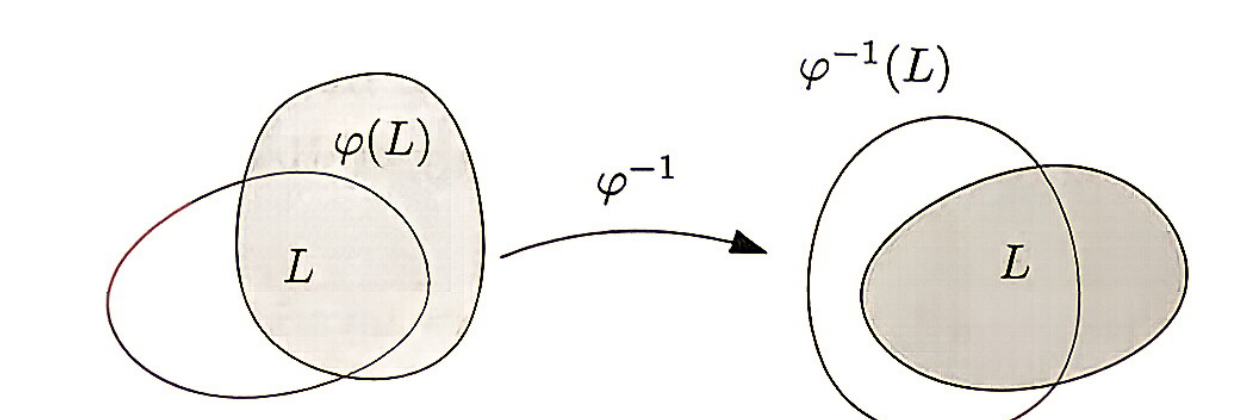
\includegraphics[width=0.7\linewidth]{figures/fig_p254_1.png}
  \caption*{图 9.6\quad 经 $\varphi^{-1}$ 作用（原书 p.246, Figure 9.6；PDF p.254）}
\end{figure}

\begin{enumerate}[label=(\roman*),start=4]
  \item 若 $R_L=\varnothing$，则 $\delta_{\|\cdot\|}\equiv0$。这是一个相当不平凡的
    结果。为证明它，我们需要一些准备。考虑 $M$ 中的开子集 $M\setminus R_L$（见上面
    观察 (i)），并定义 $\Ham(M,\omega)$ 的如下子集：
    \begin{equation}\tag{9.23}
      \Ham_{M\setminus R_L}:=\bigl\{\varphi_H^1\in\Ham(M,\omega)\bigm|
      \operatorname{supp}(H)\in[0,1]\times M\setminus R_L\bigr\}.
    \end{equation}
    于是我们有如下结果。
\end{enumerate}
% [Tutor Note: 原文疑误——(9.23) 中写 $\operatorname{supp}(H)\in[0,1]\times
% M\setminus R_L$，其中 $\in$ 应为 $\subset$（支撑集是一个集合，而非元素）；
% 且 $H$ 应理解为定义在 $[0,1]\times M$ 上的（依赖于时间的）哈密顿函数。此外原文
% 紧接着写「define the the following subset」，多了一个 the。译文按原文含义处理，
% 详见 qsg/notes/review_ch09a.md。]

\begin{wlem}{9.3.1}
  $\Ham_{M\setminus R_L}\subset\overline{\operatorname{Stab}(L)}$。
\end{wlem}

假设引理 9.3.1 成立。若 $R_L=\varnothing$，则
$\Ham_{M\setminus R_L}=\Ham(M,\omega)\subset\overline{\operatorname{Stab}(L)}
\subset\Ham(M,\omega)$。因此
$\overline{\operatorname{Stab}(L)}=\Ham(M,\omega)$，这蕴含
$\delta_{\|\cdot\|}\equiv0$，即上面的观察 (iv)。

因此，只需证明引理 9.3.1；这需要 Banyaga 的一个深刻结果。

\begin{wlem}{9.3.2}（Banyaga 碎片化引理 [23]）
  设 $(M,\omega)$ 是辛流形，任取 $M$ 的开覆盖 $\mathcal U=\{U_i\}_{i\in I}$。则任意
  $\varphi\in\Ham(M,\omega)$ 可分解为 $\varphi=\varphi_1\circ\cdots\circ\varphi_n$，
  其中 $\varphi_i\in\Ham_{U_i}$，即 $\varphi_i$ 可由一个紧支撑于 $[0,1]\times U_i$
  中的哈密顿函数生成。
\end{wlem}

\begin{wrem}{9.3.2}
  引理 9.3.2 是证明 $\Ham(M,\omega)$ 单性（simplicity）结果（当 $M$ 闭时，见
  定理 1.7.1）的关键步骤之一。引理 9.3.2 的其他应用可参见例如 [137]。
\end{wrem}

下面给出引理 9.3.1 的证明。
